\chapter{Analýza a realizace klientské aplikace}


Klientská aplikace, ať jde o jednoduché terminálové zpracování, nebo komplexní desktopový systém, má na jedno z prvních míst dávat realizaci pohodlného uživatelského rozhraní. V opačném případě celá aplikace ztrácí smysl, u uživatelů budou převládat negativní pocity, objeví se snaha najít něco jiného, co by víc odpovídalo jejich očekávání. S tímto je úzce provázána psychologická stránka lidí, jejich zvyklosti, zkušenosti s jinými programy, vnímání barev a jiné kognitivní aspekty. Každému z výše uvedených témat bude v dané kapitole věnována určitá část v souvislosti s návrhem \gls{is}.


% --------------------------------------------------------------------------------------------------
% Analýza uživatelů
% --------------------------------------------------------------------------------------------------

\section{Analýza uživatelů}

Všechny existující klientské aplikace mají vždy svoji cílovou skupinu lidí, které ji využívají. Cílem vývojářů a návrhářů takových aplikací je poskytnout uživatelům prostředí, které bude v ideálním případě optimální ve všech směrech. Pokud jde o úplně novou aplikaci, tak prvotní návrh (prototyp) nebude nikdy vyhovující, protože není známo jak se budou uživatelé chovat a co všechno budou využívat. V případě úspěchu prototypu se postupem času bude vytvářet komunita, která bude do jisté míry řídit směr vývoje aplikace. Pomyslným cílem každého projektu by tak měl být ideální stav -- uživatelé nic nechtějí a všechno perfektně funguje.

Aplikace implementovaná v dané práci spadá do první kategorie (prototyp). Proto se tato podkapitola věnuje základní analýze uživatelů, aby se stanovily přibližné požadavky z hlediska uživatelského rozhraní k již existující logické složce (\gls{api}).


\subsection{Psychologie percepce}

Vnímání lidí se v různých částech světa liší, protože mají odlišné písmo, zvyky, životní úroveň apod. Proto je důležité zkoumat navrhovanou aplikaci i z psychologického hlediska. Implementace klienta dané práce se soustředí na prostředí střední Evropy. Nebude počítat s \gls{rtl} rozhraním a speciálním vybavením a funkcionalitou pro zdravotně postižené osoby (poruchy percepce, pohybu apod.). 

Stejně jako v případě prvního setkání s člověkem je v aplikacích důležitý první dojem, který je v tomto případě ovlivněn například dobou inicializace programu, převládajícími barvami, formou jednotlivých elementů a dalšími faktory. Přitom negativní emoce vyvolané aplikací jsou vidět mnohem lépe, než pozitivní~\cite{tragicDesign}. Uživatelé nevnímají dobré rozhraní, protože je pro ně obvyklé z hlediska zvyklostí.

Oblasti web-designu se týkají především dva pojmy -- \gls{ux} a \gls{ui}. \gls{ux} se věnuje tomu, aby dojem uživatele z použití aplikace byl co nejvíc příjemný, jinými slovy se stará o zlepšení uživatelských zkušeností. \gls{ui} převádí tyto zkušenosti do vhodné formy a definuje základní barevné schéma. Barevná paleta se postupem času stává sekundárním identifikačním faktorem~\cite{colorTheory} aplikace. To se projevuje například ve vyhledávání programu v seznamu (v případě, že názvy jsou doprovázeny unikátním logem). Z tohoto důvodu odstíny a jejich kombinace, které jsou voleny během prvního veřejného prototypu, není vhodné kardinálně měnit, aby uživatelé nemuseli se opětovně přizpůsobovat novým podmínkám.

Dobrým příkladem z hlediska barevné palety je vizuální styl \gls{čvut}~\cite{cvutStyleGuide}. Základní barvou je zvolena modrá, jež v kombinací s formou lva se stává unikátní pro danou instituci. \gls{čvut} má i další, sekundární barvy, jež se mohou vyskytovat ve vizuálním zpracování materiálů univerzity, nebudou však s ní bezpodmínečně asociovány, pokud se použijí samostatně se stejnou formou (například bílý lev na zeleném pozadí).

Pro vizuální stránku \gls{is} byla primární barvou vybrána studená neintenzivní modrá barva přecházející do tmavší šedé, ukázku dané barvy lze vidět na obrázku~\ref{pic:style-guide}. Spolu s bílou tvoří neutrální kombinaci vhodnou pro dlouhodobou práci. Rozhraní se proto snaží dodržovat především monochromatické prostředí, které v případě nutnosti vyvolání pozornosti používá komplementární barvy -- žlutou nebo oranžovou. Sekundárními barvami pro vedlejší prvky byly zvoleny červená, zelená, stříbrná a modrá. Využívají se především na zvýraznění existence možné činnosti -- například odeslat, vytvořit --, a informování o výsledku -- úspěch, chyba, varování či zdržení.

Spolu s barvou je důležitá i forma od obecného rozvržení stránky až po formu jednotlivých elementů. V designu stránek pro cílové publikum zvyklé pro psaní \gls{ltr} jsou typické vzory F a Z~\cite{zfPatterns} uvedené na obrázku \ref{pic:dia-design-patterns}. Jedná se o obdobu zlatého řezu v umění. Informační systém se drží vzoru F, který je v tomto případě vhodnější z hlediska rychlosti poskytovaní užitečných informací.

\begin{fig:illustration}
   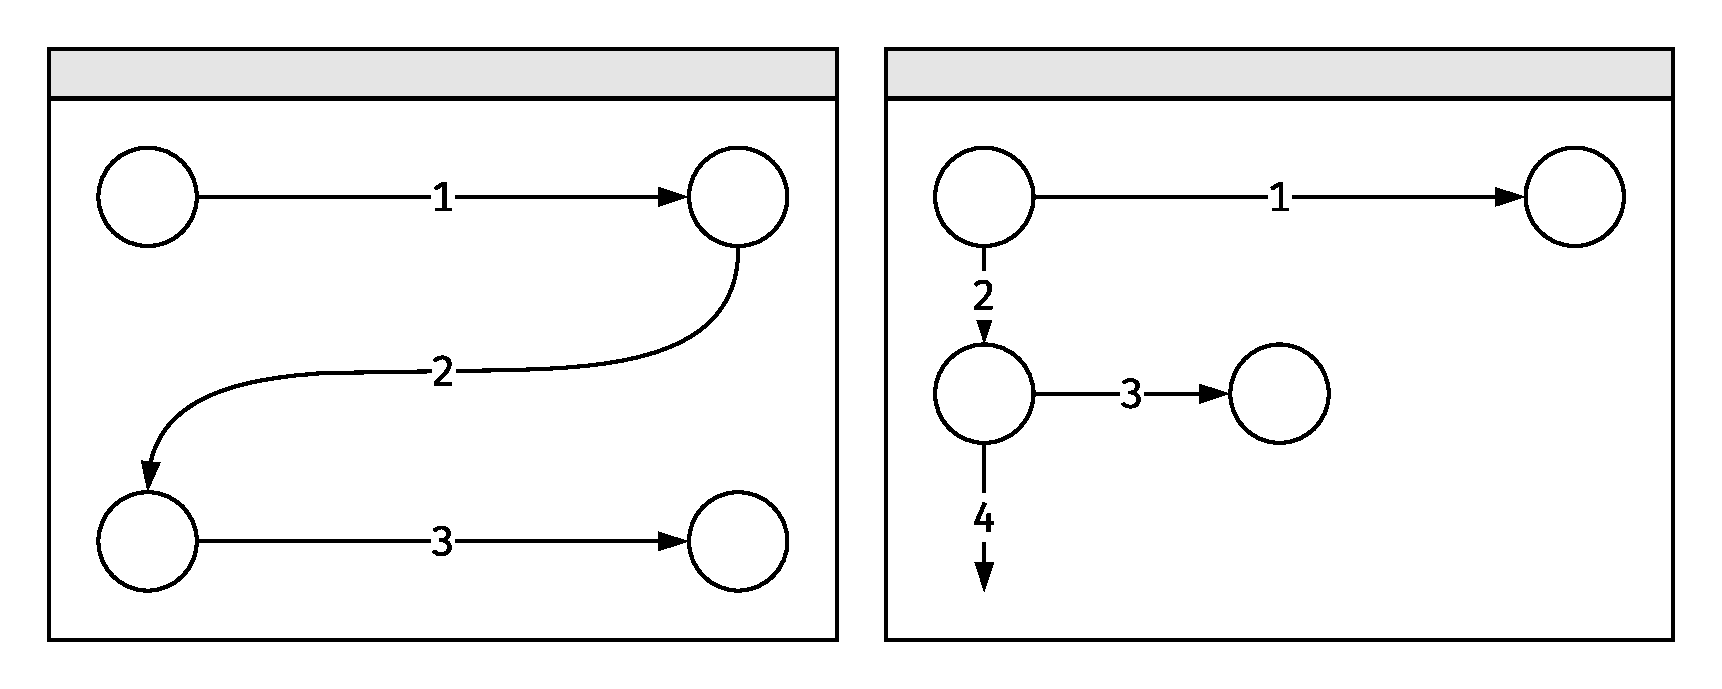
\includegraphics[width=0.8\textwidth]{images/dia-design-patterns.pdf}
   \caption{Z-vzor a F-vzor uživatelského rozhraní}\label{pic:dia-design-patterns}
\end{fig:illustration}


% --------------------------------------------------------------------------------------------------


\subsection{Cílová zařízení}

Klientské webové aplikace jsou zpravidla zobrazovány běžnými uživateli v \gls{gui} prohlížečích na zařízeních s odlišnou velikostí monitoru. Dle statistik portálu StatCounter z hlediska zařízení používanými uživateli v posledních letech převládají mobilní~\cite{statCounterDevices}. Tudíž větší zastoupení mají menší velikosti obrazovek. Z tohoto důvodu je adaptace uživatelského rozhraní \gls{is} pro mobily nutná, avšak vzhledem k povaze projektu důraz bude kladen především na desktopové velikosti obrazovek. Dle předpokladu pouze malé procento lidí bude schopno psát projekty na mobilu. Menší zařízení budou využívány pouze pro informační účely. Pokud by v pozdější době vznikla potřeba vytvořit přesnější rozhraní, tak by bylo vhodné zvážit spíš plnohodnotné mobilní aplikace, než pouze webové rozhraní. Z hlediska prohlížečů je dle obecných požadavků nutné adaptovat \gls{is} pro prohlížeče:
\begin{ulnar}
   \item Google Chrome,
   \item Mozilla Firefox,
   \item Apple Safari.
\end{ulnar}

Většina nekompatibilních funkcionalit bude řešena automaticky s pomocí podpůrných nástrojů. Mezi problémová místa bude patřit zejména přizpůsobení \gls{css} a interpretace standardů ECMAScript 6 a ECMAScript 7.


% --------------------------------------------------------------------------------------------------
% Architektira aplikace
% --------------------------------------------------------------------------------------------------


\section{Architektura aplikace}

Uživatelské rozhraní \gls{is} představuje převážně tenký klient typu webové aplikace dostupný přes webový prohlížeč. Část klientu týkající se zobrazování obsahu projektu se však blíží chování tlustého klientu, protože definuje logiku generování a vykreslování částí obsahu.

Vzhledem ke komplexním požadavkům aplikace a potřebě pokročilých funkcí základní jednoduchá implementace bez využití frameworků a knihoven není vhodná. Jednou z přijatelných variant architektury aplikace je \gls{spa} model, který je výhodný z hlediska rychlého načítání stránek a minimalizace stahovaných informací ze serveru. Negativním prvkem \gls{spa} je však velice pomalé načítání klientské aplikace. Pro první zobrazení jakékoliv stránky je nutné stáhnout celý zkompilovaný soubor aplikace, jenž v případě složitých systémů může dosahovat velikosti několika MB. Kromě načítání daného souboru je většinou ještě potřeba asynchronně dodatečně stáhnout potřebná data ze serveru přes \gls{api}. To se stává problémem na zařízeních s omezenou rychlostí připojení. Pro zobrazení čehokoliv je nutné vyčkat úplného stažení všech závislostí.

Jedním z řešení prvotního načítání jsou \gls{ssr} frameworky. Základní koncept jednotné aplikace zůstává zachovaný, avšak princip načítání první webové stránky se mění. Základní stránka s potřebnými daty je generována již na serveru a předávána jako statický \gls{html} dokument. To napodobuje chování původních webů -- uživatel dostává soubor typu \texttt{text/html}, jehož je schopen ihned zobrazit. Veškeré logické chování \gls{spa} aplikace se načítá až po zobrazení užitečného obsahu. Kromě rychlého uživatelského přístupu má toto chování i vliv na \gls{seo} indexaci stránek webovými vyhledávači. V případě daného \gls{is} však nemá význam, protože se jedná o aplikaci s chráněným obsahem.

Na základě této analýzy byla vyzkoušena implementace několika menších \gls{spa} a \gls{ssr} aplikací s využitím React a Vue. Výsledkem výběru se stal React s pomocným frameworkem pro \gls{ssr} NextJS, protože dle subjektivního hlediska byly nejvhodnější pro~realizaci daného webového klienta.

K vybraným nástrojům NextJS a React je třeba mít prostředek pro sdílení dat mezi komponentami. V základním React je tato potřeba řešena přes tzv. \uv{lifting}, který je sice jednoduchý, avšak nepřehledný. Pro předání informace z kořenové komponenty a zpět je nutné posílat potřebná data nebo funkci přes všechny mezikomponenty ve~virtuálním DOM React~\cite{reactLifting}. To vede k psaní zbytečného kódu. Místo daného způsobu lze využít jednu z knihoven pro vytváření společného úložiště. Typickým nástrojem je Redux (viz obrázek~\ref{pic:dia-redux-store}).

\begin{fig:illustration}
   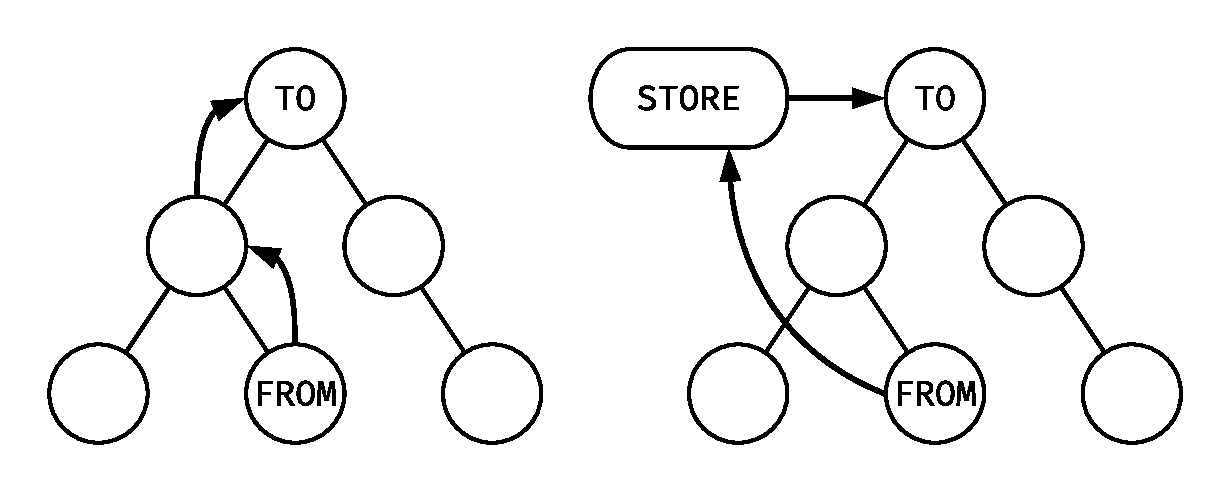
\includegraphics[width=0.8\textwidth]{images/dia-redux-store.pdf}
   \caption[Ukázka rozdílu komunikace mezi komponenty]{Ukázka rozdílu komunikace mezi komponenty bez (vlevo) nebo s (vpravo) využitím Redux}\label{pic:dia-redux-store}
\end{fig:illustration}


Z daného výběru nástrojů vyplývá, že základním jazykem pro~realizaci klientské části je JavaScript. Architektura je postavena na CommonJS a ECMAScript 6 modulech, které jsou importovány do různých částí aplikace podle potřeby. To zajišťuje přehlednost a jednoduchou podporu. Dle funkcionality lze aplikaci rozdělit do následujících vrstev:

\begin{dl}
   \item [Inicializační vrstva] Inicializační vrstva je řízena NextJS, z logického hlediska se jedná o spojení datové a prezentační vrstvy. Její chování se mění na základě prostředí, ve kterém je spouštěna (server nebo klient). Vždy stahuje a připravuje data z \gls{api} serveru, ale pokud se jedná o serverové prostředí, tak generuje i obsah typu \texttt{text/html}.
   
   \item [Prezentační vrstva] Prezentační vrstva je součástí React komponent, definuje generování prvků na webové stránce. 
   
   \item [Aplikační vrstva] Aplikační vrstva je rovněž součástí React komponent, definuje logické chování \gls{dom} elementů.
\end{dl}


\subsection{Použité technologie}

Kromě primárních frameworků zvolených během návrhu architektury pro dosažení potřebné funkcionality byly zvoleny následující nástroje a technologie:

\begin{dl}
   \item [Jazyk popisu kaskádových stylů] Základní \gls{css} je příliš přímočarý pro popis složitějších struktur. Jeho náhradou se mohly stát jazyky \gls{scss}, \gls{less}, Stylus a další, jež přidávají do \gls{css} syntaxe logické struktury -- podmínky, cykly apod. Dle subjektivních zkušeností byl zvolen \gls{scss}.
   
   \item [Vykreslování tabulek s pokročilým vyhledáváním] Pro danou funkcionalitu byly vhodné dva frameworky -- DataTables a React Table. Nejdřív byl integrován DataTables, funkcionalita vyhovovala požadavkům, avšak implementace byla náročná a nepřehledná, protože docházelo k prolínání jQuery a React syntaxe. Z tohoto důvodu byl framework DataTables nahrazen React Table.
   
   \item [Knihovna popisu rozvržení stránky] O rozvržení stránek se stará částečně importovaná knihovna Bootstrap.
   
   \item [Kompilace projektu] Kompilaci celého projektu řídí \gls{bm} Webpack, jenž je vyžadován i frameworkem NextJS. Kromě výchozích nastavení je použit pro definování \texttt{alias} proměnných kvůli přehlednějšímu importu JavaScript modulů.
\end{dl}



\subsection{Adresářová struktura}

Adresářová struktura klientské aplikace uvedená ve výpisu (viz zdrojový kód~\ref{folders:client}) se řídí požadavky frameworku \mbox{NextJS}. Složky \texttt{pages} a \texttt{static} se zdrojovými kódy nelze přesouvat do podadresářů, všechny ostatní závislosti se nachází v \texttt{src} a jsou většinou roztříděny dle typu (redux actions, redux reducers, konfigurační soubory aplikace...). Výjimku smíchaných typů zdrojových kódů tvoří složky s React komponenty -- šablony stránek a sekundární komponenty. V těchto výjimkách jsou pro přehlednost sloučeny do jedné složky JavaScript soubory komponenty a její \gls{scss} styly. Stejným způsobem jsou strukturovány i složky s jednotlivými stránkami. Bez \gls{bm} by hlídání všech závislostí v takové struktuře bylo problematické, používaný Webpack s pluginami je však nastaven pro automatické vyhledávání specifických souborů. Vývojáři zbývá pouze dodržovat určitou strukturu aplikace.

\begin{fig:code}
	\begin{minted}{text}
.
├── _templates     - šablony zdrojových kódů (stránky, redux apod.)
├── pages          - nutná složka NextJS pro stránky
├── src
│   ├── actions    - redux actions
│   ├── components - sekundární React komponenty a SCSS styly
│   ├── config     - konfigurační soubory aplikace
│   ├── layouts    - základní šablony stránek
│   ├── reducers   - redux reducers
│   ├── store      - redux store
│   ├── styles     - globální SCSS styly
│   └── utils      - utility používané v aplikaci
├── static         - nutná složka NextJS pro statické soubory
└── *.*            - inicializační a konfigurační soubory projektu
   \end{minted}
   \caption{Zkrácený výpis struktury složek klientské aplikace}\label{folders:client}
\end{fig:code}

   

% --------------------------------------------------------------------------------------------------
% Realizace funkcionalit
% --------------------------------------------------------------------------------------------------

\clearpage

\section{Realizace funkcionalit}

Převážná část webového klientu je jednoduché zobrazování dat předávaných z serverem, případně naopak volání \gls{api} metod. Na základě uživatelských informací uložených v \gls{jwt}, mezi které patří i seznam práv, se zobrazují, či naopak skrývají jednotlivé React komponenty. Jedinou implementačně zajímavou funkcionalitu tvoří zpracování částí obsahu interprety s následným generováním uživatelsky připraveného rozhraní.


\subsection{Generování obsahu projektu}
Každý založený projekt má svůj vnitřní obsah, který v průběhu existence projektu vytváří jednotliví uživatelé. Při načítání obsahu projektu uživatelem se ze serveru stahují jednotlivé části. Jedná se o struktury ve formátu \gls{json}, které obsahují data pro~generování uživatelsky přijatelného obsahu (s grafickým rozhraním) a název jednoho z interpretů obsahu (v specifikaci nazývaný jako šablona). Příklad nejjednodušší \gls{json} struktury je uveden ve zdrojovém kódu~\ref{listing:parts-json}. Proměnné \texttt{interpreter} a \texttt{store} jsou povinné pro každou část, vnitřní struktura \texttt{store} už se však řídí vybraným interpretem. 

\begin{fig:code}
	\begin{minted}{javascript}
{
   "interpreter": "text-plain",
   "store": {
      "title": "Nunc in elit",
      "text": "Pellentesque eu sapien erat."
   }
}
   \end{minted}
   \caption{Příklad JSON struktury části obsahu}\label{listing:parts-json}
\end{fig:code}

Vzhledem k tomu, že se části obsahu uchovávají v \gls{nosql} databázi, tak nejsou omezovány relacemi a přesně zadaným obsahem. Mongoose \gls{odm}, která je zprostředkovatelem spojení serverové \gls{api} aplikace a MongoDB, definuje pouze nutně potřebnou strukturu v \texttt{schema} objektech, zbytek se automaticky přizpůsobuje všem novým typem interpretů a struktury proměnné \texttt{store}. Tím je zajištěna požadovaná ohebnost obsahu.

Po načtení všech částí se generuje pole unikátních názvů interpretů, jež jsou použity v částech. Na jeho základě se s použitím nakonfigurované cesty k úložišti vkládají \mintinline{html}{<script>} tagy do \mintinline{html}{<head>} stránky. Je to potenciální místo pro útok na uživatelé systému, protože dovoluje přidat nebezpečný kód do jednoho z interpretů, který se automaticky spustí na všech zařízeních, jež ho načtou s obsahem \gls{is}. Z tohoto důvodu je nutné používat pouze úložiště s omezeným přístupem. V prototypu implementace je využíván veřejný GitHub repozitář s přístupem k souborům přes službu jsDelivr. Tato sekundární služba je nutnou součástí přístupu k souborům v repozitáři, protože \mbox{GitHub} vrací všechny soubory s \gls{mime} typem \texttt{text/html}, což znemožňuje jejich vykonávání v roli JavaScript skriptu. jsDelivr je \gls{oss} \gls{cdn} služba, která dané omezení řeší a poskytuje kopie souborů repozitáře.

\begin{fig:code}
	\begin{minted}{javascript}
(() => {
   // Unique name
   const name = 'text-plain';

   // Render function
   const render = (store) => {
      return `${store}`;
   }

   // Declare interpreter
   if(!window.iterations) window.iterations = {};
   if(!window.iterations.interpreters) 
      window.iterations.interpreters = {};
   window.iterations.interpreters[name] = {
      render
   };
})();
   \end{minted}
   \caption{Ukázka nejjednoduššího příkladu interpretu}\label{listing:interpret-js}
\end{fig:code}


Interpret v základní podobě (viz zdrojový kód~\ref{listing:interpret-js}) představuje samospouštěcí lambda funkci (tím je zajištěna ochrana vůči konfliktu globálních proměnných), jež má unikátní jméno a povinnou metodu \texttt{render}, která přijímá jako parametr \texttt{store} části obsahu a výsledkem poskytuje \gls{html} kód. Během načítání vytváří odkaz na svoje metody v globální proměnné prohlížeče \mintinline{javascript}{window.iterations.interpreters}, odkud jsou volány \gls{is}.

Podobná struktura interpretu obsahu z hlediska rozšiřitelnosti je omezena pouze možnostmi jazyka JavaScript v prostředí prohlížeče. Kromě povinné metody \mintinline{javascript}{render();} je možné definovat podpůrné funkce, manipulovat s již existujícím obsahem stránky, přidávat knihovny třetích stran, vytvářet interaktivní grafy, 3D vizualizace a další funkcionalitu.

Ve specifikaci správy obsahu \gls{is} je uveden požadavek pro návrh struktury, která by se dala rozšířit i pro komunikaci mezi jednotlivými částmi. To v daném případě lze realizovat úpravou cyklu generování obsahu. Po stažení potřebných věcí se rendering nebude provádět rovnou, před ním může být vytvářena například dočasná uživatelská databáze typu IndexedDB, která bude zprostředkovávat veškerou komunikaci. Samozřejmě bude nutné doplnit části i interprety o další povinné prvky.


% --------------------------------------------------------------------------------------------------
% Uživatelské rozhraní
% --------------------------------------------------------------------------------------------------

\clearpage
\section{Uživatelské rozhraní}

Na základě předchozích rozhodnutí o architektuře aplikace a realizace jednotlivých funkcionalit je navrženo vyhovující rozhraní. Základním východiskem je koncept plochého designu\footnote{Běžnější je anglický výraz \uv{flat design}}, jenž se projevuje ve snaze o zobrazení ovládacích prvků v přehledné, zjednodušené formě a zároveň skrytí méně potřebných funkcionalit bez většího dopadu na komfortní ovládání aplikace. Byl preferován před ostatními styly, protože obvykle nevyžaduje žádné dodatečné prvky a může být plně popsán s využitím pouze \gls{css}, tudíž je nenáročný z datového hlediska.

Před navrhováním jednotlivých stránek byl vytvořen grafický manuál\footnote{Zde je přesnější anglický výraz \uv{style guide}}. Jedná se o pomocnou stránku obsahující všechny základní prvky vyskytující se v designu -- barevná paleta, styly textů, nadpisy, prvky formulářů apod. Ukázku části manuálu lze vidět na~obrázku~\ref{pic:style-guide}, elektronická verze\footnote{Pro všechny grafické návrhy uživatelského rozhraní je využíván program Adobe XD} je dostupná v příloze této práce.

\begin{fig:illustration}
   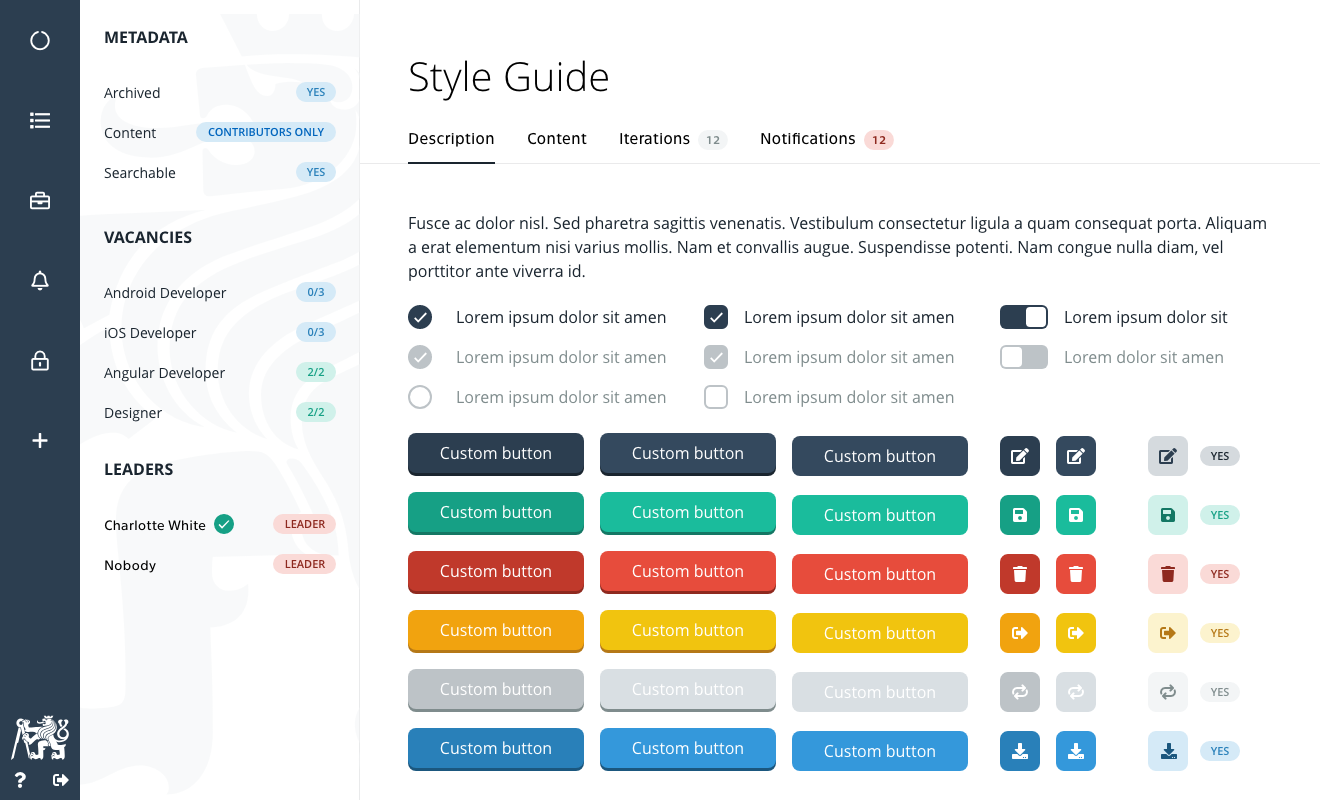
\includegraphics[width=1\textwidth]{images/style-guide.png}
   \caption{Ukázka části grafického manuálu s aplikovaným stylem pro České vysoké učení technické v Praze}\label{pic:style-guide}
\end{fig:illustration}